\documentclass[12pt, twoside, openright]{report}
\usepackage[french]{babel}
\usepackage{xltxtra}
\setmainfont[Mapping=tex-text]{Linux Libertine O}
\usepackage{amsmath}
\usepackage{graphicx}
\usepackage[colorinlistoftodos]{todonotes}
\usepackage[T1]{fontenc}
\usepackage{titlesec}
\usepackage{url}
\usepackage{hyperref}
\usepackage{geometry}
\usepackage{shorttoc}
\usepackage[backend=bibtex]{biblatex}
\usepackage{caption}
\usepackage{listings}
\usepackage[french,onelanguage]{algorithm2e}
\usepackage{csquotes}
\addbibresource{bibliographie.bib}
\usepackage{float}
\DeclareTextCommandDefault{\nobreakspace}{\leavevmode\nobreak\ } 
\geometry{
    paper=a4paper,
    inner=3cm,
    outer=2.5cm,
    top=2.5cm,
    bottom=3.5cm
}

\setcounter{secnumdepth}{4}

\titleformat{\paragraph}
{\normalfont\normalsize\bfseries}{\theparagraph}{1em}{}
\titlespacing*{\paragraph}
{0pt}{3.25ex plus 1ex minus .2ex}{1.5ex plus .2ex}
\lstdefinestyle{customc}{
  belowcaptionskip=1\baselineskip,
  breaklines=true,
  frame=L,
  xleftmargin=\parindent,
  language=C,
  showstringspaces=false,
  basicstyle=\footnotesize\ttfamily,
  keywordstyle=\bfseries\color{green!40!black},
  commentstyle=\itshape\color{purple!40!black},
  identifierstyle=\color{blue},
  stringstyle=\color{orange}
  %xleftmargin=.4
}

\begin{document}

\begin{titlepage}

\newcommand{\HRule}{\rule{\linewidth}{0.5mm}} 
\center
 

\textsc{\LARGE Nanterre université}\\[1.5cm]
\HRule \\[0.4cm]
{ \huge \bfseries Détection de la complexité algorithmique d'une fonction à partir de son code source }\\[0.4cm]
\HRule \\[1.5cm]
 \textsc{\Large Mémoire }\\[0.5cm]

\begin{minipage}{0.4\textwidth}
\begin{center} \large
\emph{Auteur:}\\
Baptiste \textsc{Rayer} 36003587
\end{center}
\end{minipage}\\[0.5cm]

\begin{minipage}{0.4\textwidth}
\begin{center} \large
\emph{Tuteur:} \\
François \textsc{Delbot}
\end{center}
\end{minipage}\\[4cm]


\includegraphics[width=10cm,height=2.25cm]{img/UPN.jpg}
\\[2cm]
\begin{center}
2018-2019    
\end{center}


\vfill 

\end{titlepage}

\newpage

\shorttoc{Sommaire}{1}

\chapter{Introduction}

\section{Motivation}
Aucune 
\section{Objectifs du mémoire}

\chapter{La complexité algorithmique}

Avant de pouvoir comprendre ce que la complexité algorithmique signifie, il est nécessaire d'avoir un idée plus globale du fonctionnement d'un outil informatique. Pour ce faire, Alan Turing a défini, en 1936, un concept qui peut nous permettre de mieux appréhender le fonctionnement d'un ordinateur.

\section{La machine de Turing}

\subsection{Définition}

La machine de Turing est un modèle théorique créé par Alan Turing en 1936. \cite{machineTuring01} Elle a pour but de définir la calculabilité d'un algorithme.   
Une machine de Turing est composée de trois éléments. (Cf: Figure \ref{fig:turing-1})
\begin{enumerate}
    \item Une unité centrale capable de dérouler le programme qui doit être exécuté par la machine. Son contenu dépend du programme à exécuter.
    \item Une bande mémoire que l'on représente par une bande en papier et qui est d'une taille infinie. C'est d'ailleurs pour cela que la machine de Turing reste une théorie. Un ordinateur de nos jours possède des centaines de giga-octets d'espace, mais nous ne sommes jamais à l'abri d'un débordement de mémoire. C'est un problème impossible à rencontrer avec une bande mémoire de taille infinie. Cette bande mémoire est découpée en cases numérotées par des entiers relatifs. C'est sur cette bande mémoire que les résultats et les calculs seront écrits. 
    \item Un pointeur qui permet la lecture et l'écriture sur la bande mémoire. Ce pointeur agit conformément aux instructions de l'unité centrale. C'est cet élément qui fait le lien entre les deux autres.
\end{enumerate}

\begin{figure}
    \begin{center}
        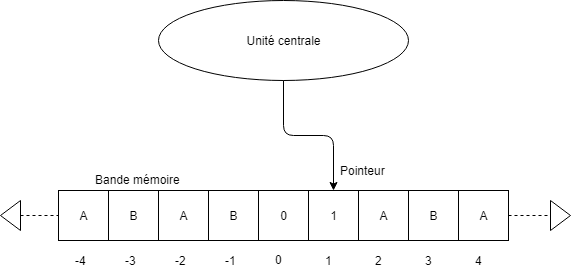
\includegraphics[height=8cm,width=12cm]{MachineDeTuring/MachineDeTuring.png}
        \caption{Représentation d'une machine de Turing}
        \label{fig:turing-1}
    \end{center}
\end{figure}
La machine de Turing dispose aussi d'un ensemble fini \textbf{S} de symboles. Il s'agit de la liste des caractères capables d'apparaître dans une case de la bande mémoire. Nous retrouvons aussi un caractère spécial ayant pour but de représenter un espace dans la bande. Nous disposons par ailleurs d'un ensemble \textbf{E} d'états possibles pour la machine de Turing. Enfin, nous avons une fonction de transition \textbf{t} qui permet de définir ce que la machine doit faire à chaque étape.

Il existe deux types de machine de Turing. D'un côté la machine de Turing déterministe qui pour chaque état possède une action à effectuer, et une valeur pour faire avancer ou reculer le pointeur. Cette action permet d'affecter une nouvelle variable à la case mémoire pointée par le pointeur. De l'autre nous avons la machine de Turing non déterministe. Pour cette machine, il est possible d'avoir plusieurs actions disponibles pour la machine et ou plusieurs valeur pour déplacer le pointeur. L'action effectuée sera donc choisie aléatoirement par la machine.

Nous nous intéresserons donc au fonctionnement d'une machine déterministe afin de déterminer la calculabilité d'une fonction. 

\subsection{Fonctionnement d'une machine de Turing déterministe}

Dans le cas d'une machine de Turing déterministe, la fonction de transition \textbf{t} peut être écrite ainsi : 
\[t = E * S * \{e', s', d\}\]
Nous retrouvons donc :
\begin{itemize}
    \item \textbf{E}, l'état actuel de la machine.
    \item \textbf{S}, le symbole courant.
    \item \textbf{e'}, l'état après exécution de \textbf{t}.
    \item \textbf{s'}, le symbole qui va remplacer \textbf{S}.
    \item \textbf{d}, le changement de position du pointeur sur la bande (typiquement 1 ou -1).
\end{itemize}

Afin d'illustrer cette définition je vais modéliser une machine simple. Elle aura pour but de transformer les caractères A en B et B en A sur les cases paires dans la bande mémoire. Si la machine rencontre deux caractères C à la suite elle s'arrête.

Nous avons donc comme dictionnaire de données : \{A, B, C\}. Nous considérerons qu'il n'y a pas de caractères vides dans la bande.

\begin{center}
    \begin{tabular}{|c|c|c|c|}
        \hline 
t        &A  & B & C \\ 
        \hline 
e1        &$(e2, B, 1)$   & $(e2, A, 1)$  & $(e4, C, 1)$  \\ 
        \hline 
e2        & $(e1, A, 1)$  & $(e1, B, 1)$  & $(e3, C, 1)$  \\ 
        \hline 
e3        &$(e2, B, 1)$  & $(e2, A, 1)$  & $-$ \\ 
        \hline 
e4        &$(e1, A, 1)$   & $(e1, B, 1)$  &  $-$\\ 
        \hline 
    \end{tabular}
    \captionof{table}{Représentation d'une machine de Turing\newline}
\end{center}

\begin{itemize}
    \item \textbf{e1, e3}, inverse A et B.
    \item \textbf{e2, e4}, avance le pointeur d'une case dans la bande sans modifier A et B. 
    \item \textbf{e3, e4}, si C est rencontré alors l'algorithme s'arrête, sinon il exécute e1 ou e2.
\end{itemize}

\section{Vitesse d'exécution et nombre d'opération élémentaire}
%Faire le lien entre machine de Turing et ordi actuel (MT restreinte mémoire finiepar exemple)
Le but d'une étude sur la complexité algorithmique d'une fonction est de pouvoir comparer deux fonctions différentes. Il existe plusieurs points de comparaison entre deux fonctions. D'un côté nous avons le temps d'exécution de la fonction, à savoir laquelle des deux est la plus rapide pour se terminer. De l'autre l'espace mémoire utilisé par la machine lors de l'exécution de ces fonctions. 



\subsection{Évolution de la vitesse de calcul des ordinateurs}

\subsubsection{Loi de Moore}

La loi de Moore énoncée par Gordon Moore, annonce que, toutes les deux années, le nombre de transistors présents dans les micro-processeurs des ordinateurs doublerait. Un transistor est un élément primordial des composants électroniques et des circuits logiques. Avec le doublement du nombre de transistors dans les micro-processeurs, la puissance de ceux-ci augmente drastiquement et un plus grand nombre d'opérations peut être effectué. Cette loi est approximativement suivie depuis qu'elle à été énoncée. Cependant avec les dernières versions des transistors, nous arrivons à une taille tellement petite par transistor, qu'il est extrêmement difficile de pouvoir réduire leurs tailles afin d'augmenter le nombre de transistor. Suite à ces problèmes, le PDG de Intel, un constructeur de micro-processeur, annonce maintenant que cette durée est passée à 2.5 ans.\cite{moore01} 

Avec toutes ces évolutions, comparer le temps d'exécution du même programme ne peut pas être fait entre deux machines différentes. Cependant, les codes peuvent être comparés autrement que par leurs durées d'exécution.

%%%Avec les changement de vitesse d'execution il faut quelque chose pour comparer les algo. C'est pour cela qu'on retrouve la notion de complexité. Qui n'évalue plus la vitesse mais le nb d'opération.%%%

\subsubsection{Définition de la complexité }

\subsection{Définition d'une opération élémentaire} %%%TODO%%%

Afin de pouvoir définir la complexité algorithmique je vais définir une opération élémentaire. Précédemment j'ai montré qu'il était impossible de comparer l'exécution d'un code d'un ordinateur à un autre. Cependant chaque ordinateur contient les même types de composants, mémoire RAM, carte mère, stockage de données ... Le matériel qui effectue les calculs dans un ordinateur correspond au processeur.  
Être capable d'identifier la perf d'un algo peut import les specs d'un ordi
Permet de comparer de manière théorique et non plus pratique.

\section{Évolution asymptotique du nombre d'opérations élémentaires}

Lorsque l'on analyse un algorithme dans des cas extrêmes, nous avons tendance à simplifier le nombre d'opérations effectuées par l'algorithme. En effet, l'étude de l'ordre de grandeur de celui-ci est plus pertinente que le fait de calculer le nombre exacts d'opérations. Ce calcul, en plus d'être complexe et de consommer beaucoup de ressources, n'apporte que peu d'informations dans le cas où les données sont de taille suffisamment grande. Pour illustrer mes propos, observons le graphique suivant.

\begin{figure}[H]
    \centering
    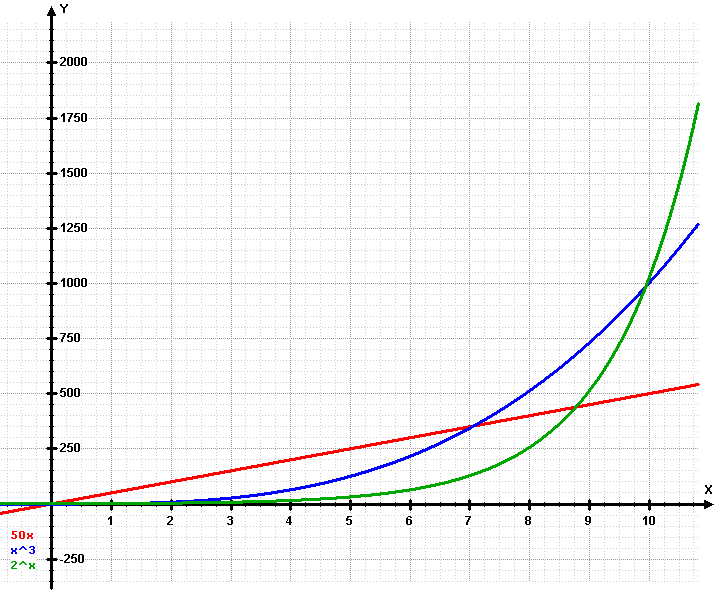
\includegraphics[height=10cm,width=14cm]{Complexite/Exponential.png}
    \caption{Représentation de trois fonctions}
    \label{fig:my_label}
\end{figure}

Sur ce graphique, nous pouvons observer trois courbes.

\begin{enumerate}
    \item En rouge, $f(x)=50y$
    \item En bleu, $f(x)=y²$
    \item En vert, $f(x)=n^{y}$
\end{enumerate}

On remarque rapidement que malgré un nombre très important, pour le facteur de la première fonction, la deuxième devient supérieure à partir de $x>=7$. Et selon la même logique, nous pouvons observer que la troisième fonction est supérieure pour $x>=11$. 

Cette observation nous permet de déterminer que si deux algorithmes ne sont pas du même ordre de grandeur, il n'est pas nécessaire de calculer un nombre précis d'opérations pour les comparer.

Dans le tableau suivant nous retrouverons des exemples d'ordres de grandeur d'algorithmes.  \cite{moore02} 
\begin{center}
    \begin{table}
        \begin{tabular}{|c|c|c|}
            \hline 
    Temps & Type & Exemple \\ 
            \hline 
    $O(1)$        &Complexité constante&  Accès à une case d'un tableau\\ 
            \hline 
    $O(log(n))$       & Complexité logarithmique  & Recherche dichotomique \\ 
            \hline 
    $O(n)$        & Complexité linéaire & Parcours d'une liste \\ 
            \hline 
    $O(n^{2})$        & Complexité quadratique  & Tri à bulle \\ 
            \hline 
    $2^{O(n)}$ & Complexité exponentielle & Brute force sur le problème du voyageur de commerce \\
            \hline
        \end{tabular}
    \caption{\label{table:complexite}Ordre de grandeurs du nombre d'opérations exécutées par un algorithme}
    \end{table}
\end{center}

Maintenant que nous comprenons qu'un ordre de grandeur est utile pour comparer deux algorithmes, comment calculer précisément le nombre d'opérations faites par une machine lors de l'exécution de ces algorithmes ? Lors de la rencontre d'un if, que doit-on choisir comme parcours ? Doit-on entrer dans le cas ou la condition est vraie ? Au contraire, faut-il analyser les deux résultats et faire la moyenne ? Dans la section suivante, nous déterminerons que la réponse à ces interrogations dépend de la complexité qui nous intéresse.

\section{Les différents types de complexité}

\subsection{En meilleur cas}

La complexité en meilleur cas consiste en l'étude d'un algorithme lorsque tous les éléments sont favorables à celui-ci. Par exemple sur un algorithme de tri de tableau, le tableau en entrée sera déjà trié. Afin de calculer le nombre d'opération effectuées lors d'une étude en meilleurs cas, il est nécessaire de suivre toutes les routes de l'algorithme contenant le moins d'opérations. 

Cette complexité permet de répondre à la question : "Quelle est la durée minimale d'exécution de mon algorithme ?". Un développeur pourras calculer la durée de réponse en meilleurs cas. Mais si à partir de ce calcul, le temps excède le maximum demandé, le développeur devra utiliser un autre algorithme plus performant afin de répondre à la problématique de son application. 

\subsection{En moyenne}

%%% https://www.researchgate.net/publication/220112145_Mean_analysis_of_an_online_algorithm_for_the_vertex\_cover\_problem/download  En moyenne necessite des outil mathématique d'analyse qui ne sont pas triviaux. Par exemple les séries génératrices ou  \url{https://fr.wikipedia.org/wiki/Transformation\_de\_Laplace}  %%%

La complexité en moyenne peut être considérée comme étant la plus représentative d'un cas réel. Un utilisateur souhaitant trier un tableau ne connaît pas forcément le contenu exact du tableau en entrée. Si il exécute plusieurs fois la fonction de tri avec des tableaux différents, il souhaite pouvoir avoir une idée du temps de réponse de l'algorithme. Cependant, l'étude de cette complexité repose sur des problèmes de distribution.

Un problème de distribution correspond à une paire entre un problème de décision et une collection de distribution. Historiquement, l'étude de la complexité en moyenne analysant des problèmes ayant des chances équiprobables.\cite{avgComplexity02} C'est-à-dire que chaque entrée avait la même probabilité de se produire. Nous ne pouvons pas considérer de nos jours que toutes les entrées d'une fonction soient équiprobables. Il faudrait déterminer la probabilité de chaque cas et, pour ce faire, une étude statisticienne de la fonction est nécessaire. L'objectif de ce mémoire n'est pas d'automatiser une étude des fonctions afin de déterminer la probabilité des valeurs d'entrée mais plutôt de calculer la complexité algorithmique de la fonction.

\subsection{Pire cas}

\subsubsection{Présentation}

L'analyse de la complexité en pire cas correspond au cas où le jeu de données sera le moins favorable à l'algorithme. Cette complexité est importante lorsqu'un système doit répondre en un temps donné. Il s'agit d'une problématique fréquente dans les systèmes embarqués, par exemple dans un outil permettant de calculer les résultats de capteurs. Dans cette optique, analyser la complexité en pire cas permet d'estimer si, avec une machine spécifique, l'algorithme terminera son travail dans les temps. 

\subsubsection{Évaluation du nombre d'opérations en pire cas}

Afin de calculer le nombre d'opérations en pire cas il faut tout d'abord déterminer quelles sont les "routes" possibles que les données peuvent emprunter dans le code.

A partir de ces chemins différents il est nécessaire de calculer le nombre d'opérations effectuées pour chacune de ces routes et de choisir celles qui contiennent le plus d'opérations. Pour information, dans le code suivant, nous avons un total de trois opérations.

\lstinputlisting[caption=Code d'une affectation de variable avec trois opérations, captionpos=b, style=customc ]{Ast/assignement.c}

La première opération est la multiplication de i par 2. Cette opération est suivie par un ajout de 7 au calcul précédent. Nous avons donc deux opérations. La troisième opération correspond à l'affectation du résultat de ces deux opération à la variable i. 

Dans le cas où une instruction élémentaire aurait un coût i, nous noterons le nombre d'opérations effectuées lors de l'exécution de la fonction 
\[{C(i)=1}\]

Le coût d'exécution d'une fonction \textbf{f} comprenant deux instructions  \textbf{i}, \textbf{j} peut être calculé par le calcul suivant : 
\[{C(i,j)=C(i)+C(j)}\]

Jusqu'ici il s'agit de la méthode de calcul simple. La première spécificité du calcul du nombre d'opérations en pire cas vient lors des conditions. Le nombre d'opération en pire cas d'une condition est égale au plus grand nombre d'opérations entre la fonction dans le if et la fonction dans le else. Considérons une condition simple que nous nommerons COND. Si la condition est valide nous exécutons le code \textbf{IF()} sinon nous exécutons le code \textbf{ELSE()} Le nombre d'opérations de cette condition peut être écrit ainsi :
\[{C(COND)=Max(C(IF()), C(ELSE())}\]

Le calcul du nombre d'opérations effectuées pire cas d'une itération est fait par la somme des opérations du code exécuté dans la boucle multipliée par le nombre d'itérations maximales de la boucle. Prenons une itération et nommons la \textbf{ITER}. Cette itération a pour maximum de nombre d'itérations \textbf{n}. Dans cette itération nous exécuterons le code de la fonction nommée \textbf{FUNC}.
\[{C(ITER)= \sum_{n=0}^{n-1} C(FUNC)}\]

A partir de ces quatre modèles de calcul il devient possible de déterminer le nombre d'opérations effectuées en pire cas de la majorité des fonctions.

\subsection{Apport de ces différentes complexités}

Avec les calculs de chaque complexité, le développeur peut apprendre le comportement de son algorithme. Il peut borner ces résultats, définir en moyenne quel est le temps de réponse de son algorithme. Cela permet de décider de manière pratique quelle est la meilleure procédure à implémenter dans son code. 

Grâce à ces calculs, il peut montrer des métriques afin de pouvoir comparer deux algorithmes, et convaincre son entourage de l'algorithme qui est le plus favorable dans le cas courant.

Il reste notable qu'en informatique théorique, ces trois types de complexité ne sont pas les seuls qui existent. Nous pouvons notamment retrouver des études sur la complexité paramétrée, qui s'occupe de rechercher la complexité d'un algorithme en fonction des paramètres au lieu de la taille de ces paramètres. 

Cependant, il existe une grande différence entre un outil qui a été développé et un algorithme. Ce qui intéresse un développeur c'est de savoir si son outil répondra dans les temps. Pour comprendre cela, nous allons présenter les différences entre un algorithme et son implémentation dans le chapitre suivant.

\chapter{Complexité et code source}

\section{Un algorithme en pseudo-code}

Il est important de rappeler qu'un algorithme n'est pas une implémentation. Prenons la définition du dictionnaire. Algorithme : Ensemble de règles opératoires dont l'application permet de résoudre un problème énoncé au moyen d'un nombre fini d'opérations. Un algorithme peut être traduit, grâce à un langage de programmation, en un programme exécutable par un ordinateur.\cite{algorithme01} Cet ensemble de règles ne permet pas de résoudre un cas pratique, un problème particulier, mais donne les indications pour créer un code permettant de résoudre ce cas. Prenons l'algorithme du tri à bulle. 

\vspace{0.4cm}

\begin{algorithm}[H]
    
    \KwData{$tab, taille$ Un tableau ainsi que la taille de ce tableau}
    \KwResult{Un tableau trié}
    
    \For{$i$ allant de $taille-1 à 1$}
    {
        \For{$j$ allant de $0$ à $i-1$}
        {
            \If{$tab[j+1] < tab[j]$}
            {
                échanger($tab[j+1], tab[j]$)
            }
        }
    }
    \caption{Tri à bulle($tab, taille$)}
\end{algorithm}
 \vspace{0.4cm}
Ici nous avons l'équivalent d'une recette de cuisine avec comme ingrédients : les variables et la recette, la méthode de programmation. Ce pseudo-code correspond à un langage abstrait qu'un humain pourra interpréter et implémenter sous la forme d'un code. Pour conclure, il est important de comprendre qu'un algorithme n'est pas une spécification formelle. Différents développeurs suivant un algorithme obtiendront différents codes en fonction de leurs implémentations.

\section{Un même algorithme, plusieurs variations}

Nous pouvons observer aussi qu'il existe pour un même algorithme plusieurs façon de l'écrire dans un langage commun. Reprenons le tri à bulle. Il s'agit d'un algorithme permettant de trier un tableau. Ce tri lit les éléments du tableau par ordre croissant des indices et inverse les nombres qui ne sont pas ordonnés.

\lstinputlisting[caption=Tri à bulle en C, style=customc]{CodeSource/triabulle.c}

Mais rien n'empêche le développeur de trier le tableau dans le sens inverse. Il peut commencer à lire le tableau par les indices descendants, l'algorithme utilisé reste le même. Cela parait anodin comme changement mais les répercussions sont importantes dans le code. Par exemples, les conditions des itérations changent entièrement.

\lstinputlisting[caption=Tri à bulle triant dans le sens inverse, style=customc]{CodeSource/triabulleinverse.c}

Dans le premier cas, il est facile en observant la condition de savoir combien d'itérations la boucle va faire, et quelles variables sont impliquées dans le calcul de la complexité. Dans le cas précédent nous pouvons observer que la variable \textit{taille} est l'élément clé de ces itérations. Dans le second cas, il est impossible de déterminer la variable impliquée dans celles-ci à partir de la condition. Il est nécessaire d'observer les initialisations des variables pour se rendre compte que la variable \textit{taille} est l'élément clé de ces itérations.

Nous venons de montrer que pour un algorithme, nous pouvions retrouver plusieurs interprétations. Chaque interprétation de cet algorithme conduit donc à des codes différents. Mais pour la même interprétation d'un algorithme, il est possible d'avoir un code différent. Dans le tri à bulle, nous retrouvons des boucles qui itèrent sur les élément d'un tableau. Les développeurs ont accès à trois structures de contrôle pour effectuer les itérations en c : \textit{for} \textit{while}, \textit{do while}. Le code est différent entre ces trois cas bien que l'algorithme soit identique. 


\subsection{Évaluation de la complexité d'un algorithme}

\subsubsection{Terminaison d'une fonction : un problème indécidable}

En 1936, Alan Turing prouve qu'il n'est pas possible de déterminer à partir d'un programme informatique si un autre programme s'arrête. Il détermine donc qu'il s'agit d'un problème indécidable.

%%%TODO c'est du copié collé ATM de \cite{codesource02}%%%
Il est donc impossible de déterminer dans tous les cas possibles si un programme est fini. 
\begin{enumerate}
    \item automatique (sans intervention humaine, annotation, etc.) ;
    \item correcte (sound — elle ne donne pas de résultats faux) ;
    \item complète (complete — elle est capable de prouver tous les résultats
    vrais) ;
    \item non limitée à des exécutions ou des mémoires bornées.
\end{enumerate}
\cite{codesource02} théorème de Rice

\subsubsection{Exemple d'évaluation de la complexité en pire cas d'un algorithme}

%%%Extraire une formule qui dépend de taille. La complexité est donc en lien avec la valeur de taille. Puis dire que l'objectif de mémoir c'est d'automatiser ce qui vient d'être fait à la main sur une fonction simple => probleme d'indécadibilité obligation de se résoudre à utiliser un sous langage Trop restreint pas d'algo interessant, pas assez pas de bonnes automatisation%%%

Reprenons le code C du tri à bulle. Je vais à présent dérouler la méthode vue en 2.4 afin de calculer le nombre d'opérations élémentaires effectuées en pire cas pour ce code C. 

Nous avons dans un premier temps trois déclarations de variables, ce qui correspond à trois opérations élémentaires exécutées peu importe les données envoyées ce qui correspond donc à une complexité constante \[C(3)\]

Je vais ensuite calculer le nombre d'opérations élémentaires du code qui se trouvent à l'intérieur de la condition et des deux itérations. A la première ligne de ce code nous avons une affectation de valeur soit une opération élémentaire. A la deuxième et à la troisième ligne, nous retrouvons deux opérations élémentaires. La première, l'affectation de variable et la deuxième le calcul de j+1. Nous obtenons donc un total de cinq opération élémentaires, soit \[C(5)\]

Maintenant ajoutons la condition. La condition représente à elle seule deux opérations élémentaires, une pour j+1 et une pour la comparaison entre deux variables. La condition ne possède pas de else, et donc ne donne pas d'instructions supplémentaires si la condition n'est pas valide. Comme nous cherchons le pire cas, nous allons considérer que la condition est toujours invalide. Nous obtenons donc pour cette condition en pire cas sept instructions élémentaires pour une complexité toujours constante de \[C(7)\] 

Je vais maintenant ajouter le calcul de la deuxième itération. Cette itération est composée d'une affectation effectuant une opération élémentaire. Cette affectation n'est effectuée qu'une fois, à l'initialisation de la boucle. Nous avons une incrémentation de la variable y qui est exécutée autant de fois que la boucle itère. Ensuite nous avons la condition de l'itération qui elle aussi est exécutée autant de fois que la boucle itère. Et finalement les instructions élémentaires à l'intérieur de la boucle sont répétés autant de fois que la boucle itère. Cette condition est composée de deux opérations élémentaires : le calcul de taille - 1 et la comparaison entre j et le résultat de ce calcul. Nous avons donc  : $1 + (1 + 2 + 7) *$ nombre d'itérations de la boucle  opérations élémentaires. En observant la condition de la boucle ainsi que l'initialisation des variables, nous pouvons en déduire que le nombre d'opérations élémentaires est de $ 1 + 10 * (taille - 1)$. Pour obtenir la complexité en pire cas, nous considérerons donc que la boucle est exécutée le maximum de fois. Nous observons donc notre premier changement d'ordre de grandeur dans la complexité de la fonction. En effet nous n'avons plus une complexité constante mais une complexité dépendante de la variable taille. La boucle étant répétée \textit{taille} fois , nous avons une complexité qui est maintenant linéaire : \[C(1 + 10 * (taille-1))\] 

Elle est réductible par ordre de grandeur à \[O(10*taille) => O(taille)\]

En appliquant le même procédé pour la première boucle, nous observons un nombre d'opérations élémentaires égal à $1 + (2 + 1 + $nombre d'opérations internes à la boucle $) *$ nombre d'itérations de la boucle. A nouveau nous pouvons déterminer le nombre d'itérations de cette boucle : la boucle itère taille fois. 

Nous avons maintenant tous les éléments nécessaires pour calculer le nombre d'opérations élémentaires en pire cas, et ensuite déterminer la complexité en pire cas de cette fonction. 
$$ 4 + ( 3 + (10 * (taille - 1))) * taille$$
Ce qui nous donne une complexité en pire cas de 

\[C(4 + (3 + (10 * (taille - 1))) * taille)\] 

Elle peut être réduite en : \[O((10*taille) * taille) => O(taille^{2})\] 

 Il s'agit donc visiblement d'une complexité quadratique.(Cf: \ref{table:complexite}) La complexité est donc fortement liée à la taille. L'objectif de ce mémoire est d'automatiser ce procédé. Cependant comme nous l'avons vu auparavant avec le théorème de Rice, il est inconcevable de pouvoir faire une automatisation possible pour tous les cas ; ce n'est pas une solution viable. Pour cela, et avant de déterminer un sous langage qui permette de travailler sur un maximum de code, nous allons observer les outils existants. 


\chapter{Les outils existants}
%%%LEs outils actuels ne permettent pas de déterminer la complexité en pire cas sur tous les algo + complexité cyclomatique%%%
%%% TODO: mini intro à ce chapitre%%% 


\section{Manipulation du code source}

\subsection{Arbre syntaxique}

Un arbre de syntaxe abstraite est une représentation du code. Il s'agit d'un graphe ayant comme noeud chaque interaction du code. Je vais présenter à titre d'exemple deux types n\oe{}uds que nous pouvons retrouver dans un code.

\subsubsection{Les n\oe{}uds opération binaire}

Ces n\oe{}uds représentent tous les calculs dans les outils. Ils sont représentés par trois éléments : un côté droit, un côté gauche et un opérateur. Les deux côtés de l'opération peuvent être représentés par une nouvelle opération binaire. L'opérateur est la méthode de calcul entre les éléments gauche et droit, par exemple +, -, /, *, \% etc. Nous pouvons donc écrire le code suivant :

\lstinputlisting[caption=Code d'une affectation de variable, style=customc]{Ast/assignement.c}
Sous la forme de l'arbre syntaxique suivant : 
\begin{center}
    \begin{figure}[H]
        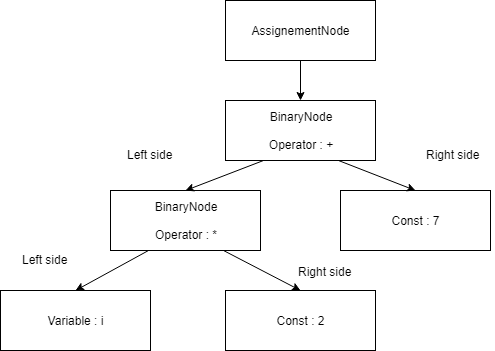
\includegraphics[height=8cm,width=12cm]{Ast/ASTBinaryNode.png}
        \caption{Arbre syntaxique du n\oe{}ud binaire}
    \end{figure}
\end{center}

\subsubsection{Les n\oe{}uds conditionnels}
Ces n\oe{}uds correspondent aux conditions ; ils sont composés de plusieurs sous n\oe{}uds. Le premier est un n\oe{}ud d'opération binaire pour la condition. Ensuite il contient deux blocs de n\oe{}uds représentant soit le cas où la condition est valide soit le cas où elle n'est pas respectée. Prenons le code suivant comme exemple.
    \lstinputlisting[caption=Code d'un if, style=customc]{Ast/if.c}
    Nous le retrouvons avec comme représentation sous forme d'arbre :
    \begin{figure}[H]
        \begin{center}
            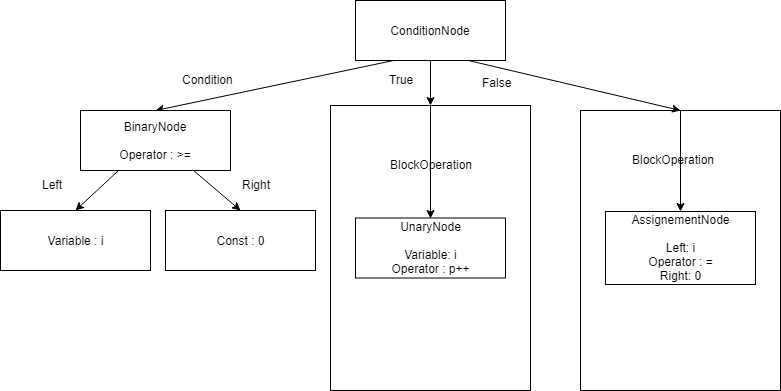
\includegraphics[height=8cm,width=14cm]{Ast/ASTIfNode.png}
            \caption{Arbre syntaxique d'un n\oe{}ud conditionnel}
        \end{center}
    \end{figure}

\section{Compilateur}

\subsection{Rappel sur les types de langages}

Nous pouvons retrouver plusieurs niveaux d'abstraction pour les langages.\cite{compilateur01}
\begin{itemize}
    \item Les langages dédiés (ou Domain Specific Language) -- tels que MatLab, SQL, etc.-- qui ont pour but de répondre à un besoin applicatif spécifique. 
    \item Les langages de haut niveaux -- comme java, c, COBOL, etc. -- qui permettent de répondre à de multiples problèmes à l'aide d'une écriture plus proche de l'humain.
    \item Les langages intermédiaires (Gimple, Bytecode Java),qui correspondent au code de transition entre les langages de haut niveau et les langages machines. Ce code est analysable par une machine abstraite afin de détecter les erreurs et d'optimiser au mieux le code machine.
    \item Les langages machines (x86, ARM), qui correspond à une suite de bits qui est compris par le processeur de la machine.
\end{itemize}

\subsection{Définition d'un compilateur}

Un compilateur est un programme informatique qui transforme un code source écrit dans un langage (le langage source) en un autre langage (le langage cible). \cite{compilateur02} Le compilateur peut donc être associé à un traducteur entre deux langages. \cite{compilateur01}

Un compilateur peut fonctionner de trois manières différentes : 
\begin{enumerate}
    \item Compilation : le compilateur traduit le langage en entrée vers le langage en sortie. Dans ce cas le résultat des deux programmes est identique.
    \item Interprétation : le compilateur prend un programme en entrée avec des données et calcule le résultat.
    \item Machine virtuelle : le compilateur traduit le langage d'entrée vers un langage intermédiaire puis interprète celui-ci.
\end{enumerate}

\section{Linter}
Les linters sont des programmes informatiques permettant d'effectuer une analyse statique sur le code. Le nom linter a pour origine l'outil \textit{lint} sur unix. Cet outil avait pour but à l'époque de compléter les compilateurs. En effet, afin d'obtenir une compilation rapide, très peu de vérifications étaient effectuées sur le code du développeur. Ainsi le lint permettait de vérifier plusieurs problèmes récurrents du code : l'initialisation ou l'utilisation de variables, le flot de contrôle, les appels de fonction, etc. \cite{linter01}

Ces fonctionnalités sont maintenant souvent présentes dans les compilateurs. Par exemple \textit{GCC} avec l'option --WALL affichera les variables non utilisées. Nous retrouvons même des plugins pour IDE qui implémentent des linters. L'utilisation d'un linter de nos jours est considérée comme une bonne pratique de développement. Les linters ne vérifient plus uniquement les erreurs possibles de code : ils prennent maintenant en compte les mauvaises pratiques de développement.  

Afin de créer un code durable et entretenable suite aux évolutions des besoins, des outils d'intégration continue ont été créés. Parmi ces outils certains, comme \textit{Codacy}, utilisent des linters afin d'analyser le code et de reporter les problèmes possibles. Avec les résultats de ces analyses, ils peuvent donner une note à un projet qui reflétera la qualité du code.   

\section{Notre choix d'outil}

PycParser => transforme le code en arbre syntaxique grâce à gcc

\chapter{Implémentation}

// EXPLICATION

\section{Restriction du langage}

Comme nous l'avons expliqué auparavant, il n'est pas possible de faire un algorithme permettant d'affirmer qu'un code se termine sans exécuter ce code. Il paraît donc évident que créer un code permettant de déterminer la complexité entière d'un algorithme est une tâche non réalisable dans un cas général. Cependant, nous ne cherchons pas à déterminer la complexité de toutes les fonctions qu'un développeur senior pourrait créer. Notre objectif est de créer un outil permettant de calculer la complexité d'un code écrit par un étudiant apprenant à développer. Cet étudiant va donc développer des fonctions relativement courtes. Cela nous permettra de mieux centrer l'objectif de notre analyseur et donc de pouvoir obtenir un résultat, là où il serait impossible d'en déterminer un dans tous les algorithmes.

Pour cela nous avons décidé d'exclure plusieurs pratiques de code et d'ignorer certaines fonctionnalités du c. Par exemple en c nous pouvons utiliser des labels et des GOTO. Cette fonctionnalité n'est pas recommandée et obfusque le code. Ce type de méthode rend beaucoup plus complexe l'analyse. Durant les enseignements, cette méthode est d'ailleurs fortement déconseillée par les professeurs. Nous allons donc ignorer les codes contenant des GOTO.

Afin de traiter de manière efficace le code, nous nous concentrerons sur des code c utilisant des types de bases. Les étudiants seront amenés, en apprenant la programmation, à créer des structures de données avec la méthode \textit{struct}. L'utilisation de ces structures peut rendre des codes complexes sans pour autant affecter l'algorithme que l'étudiant souhaite implémenter. Nous nous concentrerons donc sur des algorithmes utilisant les types primitifs du C, puisqu'un étudiant capable d'écrire un code fonctionnant avec des types primitifs sera capable de réécrire son code après analyse avec une structure, l'algorithme restant inchangé. // MAL DIT

Un autre problème complexe vient avec la gestion des pointeurs en C. Il s'agit ici d'un élément clé de ce langage. Les pointeurs, l'allocation dynamique est un rite de passage pour tout étudiant apprenant la programmation C. Cependant il est extrêmement difficile d'analyser un code utilisant des pointeurs et une gestion dynamique de mémoire. Obtenir la variable d'un code source via son adresse rend presque impossible l'étude d'un algorithme, ou nécessite de créer un outil bien trop spécifique à ce cas. Mais nous ne pouvons pas nous passer des tableaux dans un langage de programmation.  C'est pour cela que nous nous orienterons vers une analyse de code utilisant le sucre syntaxique du c sur les tableaux.

Limitation à une fonction %%%TODO%%%

\section{Proposition}



\chapter{Conclusion}

\tableofcontents
\printbibliography
\end{document}